
\section{Mathematical Formulation}\label{sec:math_formulation}

\begin{figure*}[h]
  \centering
  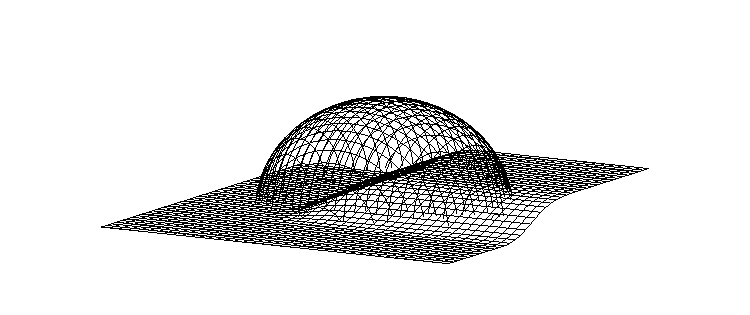
\includegraphics[height=120pt,trim=10 10 10 40,clip]{figures/surface.pdf}
  \caption{Boundary domain for the computation.}
  \label{fig:boundary_domain}
\end{figure*}

Consider a volume large enough to enclose the entire ground region that moves as a result of an underground explosion but small enough so that meterological effects can be neglected. In this volume
\[
\Big(\nabla^2+k^2\Big)P({\bf x},\omega)=0.
\]
Here $k=\frac{2\pi f}{c}$, where $f$ is angular frequency and $c$ is the speed of sound, is the wavenumber. If $B$ is the boundary of this volume then by the Kirchoff-Helmholtz integral formula \cite{morse1968theoretical}
\begin{equation}\label{eq:kirk_helm}
P({\bf x})
=
\int_{B} \bigg[
\Big({\bf \hat n}\cdot\nabla_{\bf y} G({\bf x},{\bf y})\Big)P({\bf y})
+
i\omega\rho G({\bf x},{\bf y}){\bf \hat n}\cdot{\bf v}({\bf y})
\bigg]\, d\sigma({\bf y}).
\end{equation}
for ${\bf x}$ not on the surface $B$. On the surface, for ${\bf x}\in B$, the overpressure satisfies 
\begin{equation}\label{eq:kirk_helm_P_on_surface}
c({\bf x})P({\bf x})
=
\int_{B} \bigg[
\Big({\bf \hat n}\cdot\nabla_{\bf y} G({\bf x},{\bf y})\Big)P({\bf y})
+
i\omega\rho G({\bf x},{\bf y}){\bf \hat n}\cdot{\bf v}({\bf y})
\bigg]\, d\sigma({\bf y})
\end{equation}
where $c({\bf x})$ is $\frac{1}{4\pi}$ times the solid angle ({\color{red} using a Greens' function is normalized to yield a delta function rather than a delta function over $4\pi$}) subtended by the computational volume at ${\bf x}$. 

Consider a sphere, $S$, of radius $R$ centered at the spot on the ground directly above the explosion. Choose the computational volume to be the intersection of the sphere with the region above the ground surface. Then $B=G\cup D$ where $G$ is the ground surface contained in $S$ and $D$ is the part of $S$ above the ground surface. Choosing the Green's function to have Dirichlet boundary conditions on $S$ one has
\begin{equation}\label{eq:kirk_helm_domain_dir_sphere}
\begin{aligned}
c({\bf x})P({\bf x})
=&
\int_{G} \bigg[
\Big({\bf \hat n}\cdot\nabla_{\bf y} G({\bf x},{\bf y})\Big)P({\bf y})
+
i\omega\rho G({\bf x},{\bf y}){\bf \hat n}\cdot{\bf v}({\bf y})
\bigg]\, d\sigma({\bf y})\\
&+
\int_{D} 
\Big({\bf \hat n}\cdot\nabla_{\bf y} G({\bf x},{\bf y})\Big)P({\bf y})
\, d\sigma({\bf y}).
\end{aligned}
\end{equation}
On $D$ one can use spherical coordinates $r,\theta,\phi$ and one then has $d\sigma=R^2\sin\theta\, d\theta d\phi$. On $G$, let $z=h(x,y)$ be the height of the ground, measured from the ground point directly above the explosion. Then one has 
\begin{equation}\label{eq:gnd_surface_element}
d\sigma=\sqrt{1+(\frac{\partial h}{\partial x})^2+(\frac{\partial h}{\partial y})^2\,}\, dx\, dy
\end{equation}
Note that ${\bf x}$ is inside the volume considered, and approaches the surface from the inside. In particular $\|{\bf x}\|\le R$. 

The surface velocity ${\bf v}$ is the source of the acoustic excitation in this problem. The principle of solution is to treat the above integral equation as a linear equation for the pressure $P$ on $B$ and solve for $P$. \cite{schenck1968improved,bai2013acoustic} This will be accomplished by using a version of the Galerkin method to approximate the integral equation with a linear system and then solve the linear system using a straightforward LU algorithm. Some subtleties arise in taking the limit as ${\bf x}$ approaches the surface $B$ and from singluar behavior of the Green's function at frequencies corresponding to resonances in a sphere with pressure release boundary conditions on its surface. This leads to spurious zero modes (modes with eigenvalue zero) in the resulting linear system. These subtleties are dealt with in the literature where they are called the ``nonuniqueness problem''. \cite{schenck1968improved} 

\subsection{The Green's Function:}\label{subsec:greens_func}

We construct the Green's function in sperical coordinates \cite{williams1999fourier}
\[
G(r_{\bf x},\theta_{\bf x},\phi_{\bf x},r_{\bf y},\theta_{\bf y},\phi_{\bf y})
=
\sum_{l,m}Y_{l,m}(\theta_{\bf x},\phi_{\bf x})Y_{l,m}^*(\theta_{\bf y},\phi_{\bf y})g_l(r_{\bf x},r_{\bf y})
\]
where 
\[
\Big(\secparderiv r + \frac{2}{r}\parderiv r - \frac{l(l+1)}{r^2} +k^2\Big)g_l(r,r^\prime)
=\frac{\delta(r-r^\prime)}{rr^\prime}
\]
and $k=\frac{\omega}{c}$. The radial component, $g_l(r,r^\prime)$, can be constructed out of spherical Bessel functions $j_l$ and $y_l$: 
\[
g_l(r,r^\prime)=kj_l(kr_<)\Big(y_l(kr_>)-\frac{y_l(kR)}{j_l(kR)}j_l(kr_>)\Big)
\]
where $r_<=\text{min}\{r,r^\prime\}$,  $r_>=\text{max}\{r,r^\prime\}$. 

Use can be made of the summation formula (see http://dlmf.nist.gov)
\[
\sum_{m=-l}^lY_{l,m}(\theta_{\bf x},\phi_{\bf x})Y_{l,m}^*(\theta_{\bf y},\phi_{\bf y})
=
\frac{2l+1}{4\pi}P_l\big(\cos\Omega(\theta_{\bf x},\phi_{\bf x},\theta_{\bf y},\phi_{\bf y})\big),
\]
where $P_l$ is the Legendre polynomial and $\Omega(\theta_{\bf x},\phi_{\bf x},\theta_{\bf y},\phi_{\bf y})$ is the angle between the vectors ${\bf x}$ and ${\bf y}$. Note that 
\[
\cos\Omega(\theta_{\bf x},\phi_{\bf x},\theta_{\bf y},\phi_{\bf y})=\cos\theta_{\bf x}\cos\theta_{\bf y}+\sin\theta_{\bf x}\sin\theta_{\bf y}\cos(\phi_{\bf x}-\phi_{\bf y}). 
\]
Substituting in one finds
\begin{equation}\label{eq:greens_function}
G(r_{\bf x},\theta_{\bf x},\phi_{\bf x},r_{\bf y},\theta_{\bf y},\phi_{\bf y})
=
\sum_{l=0}^\infty\frac{2l+1}{4\pi}P_l\big(\cos\Omega(\theta_{\bf x},\phi_{\bf x},\theta_{\bf y},\phi_{\bf y})\big)
kj_l(kr_<)\Big(y_l(kr_>)-\frac{y_l(kR)}{j_l(kR)}j_l(kr_>)\Big).
\end{equation}

The radial Green's function $g_l$ is singlular at frequencies for which 
\[
j_l(kR)=j_l(\frac{2\pi fR}{c})=0.
\]
The smallest zero of a spherical Bessel function is that of $j_0(x)$ at $x=\pi$ so that, for $c=340\text{ m/s}$ and $R$ in the range of hundreds of meters the lowest such frequency is around 1 Hz. At these frequencies one finds zero modes in the resulting linear system for $P$. A method (known in the literature as the CHIEF method) for handling the associated indeterminacy. Initially the code will be tested at frequencies where this is not an issue. The implementation of the CHIEF (or some other) method will be done at some later point. 

\subsection{The Normal Derivatives of the Greens' Function}

Note that, since $r_{\bf y}=R$ and $r_{\bf x}<R$ on $D$, 
\begin{align*}
{\bf \hat n}\cdot&\nabla_{\bf y} G({\bf x},{\bf y})\big|_{{\bf y}\in D}=\frac{\partial}{\partial r_{\bf y}} G({\bf x},{\bf y})\big|_{r_{\bf y}=R}
\\
&=\sum_l\frac{2l+1}{4\pi}P_l\big(\cos\Omega\big)\frac{\partial}{\partial r_{\bf y}} g_l(r_{\bf x},r_{\bf y})\big|_{r_{\bf y}=R}
\\
&=
\sum_l\frac{2l+1}{4\pi}P_l\big(\cos\Omega\big)
k^2\frac{j_l(kr_{\bf x})}{j_l(kR)}\Big(j_l(kR)y_l^\prime(kR)-j_l^\prime(kR)y_l(kR)\Big)
\\
&=
\sum_l\frac{2l+1}{4\pi}P_l\big(\cos\Omega\big)\frac{j_l(kr_{\bf x})}{R^2j_l(kR)}
\end{align*}
for ${\bf y}\in D$.

To compute the normal derivative on the ground surface $G$ one needs a parameterization of the surface. Recall that $z=h(x,y)$ is the height of the ground, measured from the ground point directly above the explosion. Then the unit normal to the ground surface is given by 
\[
{\bf \hat n}
=
\frac{1}{\sqrt{1+(\frac{\partial h}{\partial x})^2+(\frac{\partial h}{\partial y})^2}}
\begin{pmatrix}-\frac{\partial h}{\partial x}\\-\frac{\partial h}{\partial y}\\1\end{pmatrix}
\]
and
\[
{\bf \hat n}\cdot\nabla
=
\frac{1}{\sqrt{1+(\frac{\partial h}{\partial x})^2+(\frac{\partial h}{\partial y})^2}}
\Big(
-\frac{\partial h}{\partial x}\frac{\partial}{\partial x}-\frac{\partial h}{\partial y}\frac{\partial}{\partial y}
+\frac{\partial}{\partial z}
\Big).
\]
Transforming to spherical coordinates we use
\[
\parderiv x
=
\sin\theta\cos\phi\parderiv r
+
\frac{1}{ r}\cos\theta\cos\phi\parderiv \theta
-
\frac{\sin\phi}{ r\sin\theta}\parderiv \phi,
\]
\[
\parderiv y
=
\sin\theta\sin\phi\parderiv r
+
\frac{1}{ r}\cos\theta\sin\phi\parderiv \theta
+
\frac{\cos\phi}{ r\sin\theta}\parderiv \phi
\]
and
\[
\parderiv z
=
\cos\theta\parderiv r
-\frac{1}{ r}\sin\theta\parderiv \theta
\]
so that 
\begin{align*}
{\bf \hat n}\cdot\nabla
=
\frac{1}{\sqrt{1+(\frac{\partial h}{\partial x})^2+(\frac{\partial h}{\partial y})^2}}
\bigg[&
\Big(\cos\theta-\frac{\partial h}{\partial x}\sin\theta\cos\phi
-\frac{\partial h}{\partial y}\sin\theta\sin\phi\Big)\frac{\partial}{\partial r}\\
&-
\frac{1}{r}\Big(\sin\theta+\frac{\partial h}{\partial x}\cos\theta\cos\phi
+\frac{\partial h}{\partial y}\cos\theta\sin\phi\Big)\frac{\partial}{\partial \theta}\\
&+
\frac{1}{r}\Big(\frac{\partial h}{\partial x}\frac{\sin\phi}{ r\sin\theta}
-\frac{\partial h}{\partial y}\frac{\cos\phi}{ r\sin\theta}\Big)\frac{\partial}{\partial \phi}
\bigg].
\end{align*}
For ${\bf y}\in G$ on then has, with $G$ specified by $y_3=h(y_1,y_2)$, 
\begin{align*}
{\bf \hat n}\cdot\nabla_{\bf y} G({\bf x},{\bf y})
=&
\frac{1}{\sqrt{1+(\frac{\partial h}{\partial y_1})^2+(\frac{\partial h}{\partial y_2})^2}}
\sum_{l=0}^\infty\frac{2l+1}{4\pi}\\
&\bigg[
\Big(\cos\theta_{\bf y}-\frac{\partial h}{\partial y_1}\sin\theta_{\bf y}\cos\phi_{\bf y}
-\frac{\partial h}{\partial y_2}\sin\theta_{\bf y}\sin\phi_{\bf y}\Big)\frac{\partial}{\partial r_{\bf y}}\\
&-
\frac{1}{r_{\bf y}}\Big(\sin\theta_{\bf y}+\frac{\partial h}{\partial y_1}\cos\theta_{\bf y}\cos\phi_{\bf y}
+\frac{\partial h}{\partial y_2}\cos\theta_{\bf y}\sin\phi_{\bf y}\Big)\frac{\partial}{\partial \theta_{\bf y}}\\
&+
\frac{1}{r_{\bf y}}\Big(\frac{\partial h}{\partial y_1}\frac{\sin\phi_{\bf y}}{ r\sin\theta_{\bf y}}
-\frac{\partial h}{\partial y_2}\frac{\cos\phi_{\bf y}}{ r\sin\theta_{\bf y}}\Big)\frac{\partial}{\partial \phi_{\bf y}}
\bigg]P_l(\cos\Omega)g_l(r_{\bf x},r_{\bf y}).
\end{align*}
One has 
\[
\frac{\partial}{\partial r_{\bf y}}g_l(r_{\bf x},r_{\bf y})
=
k^2\begin{cases}
j_l(kr_{\bf x})\Big(y_l^\prime(kr_{\bf y})-\frac{y_l(kR)}{j_l(kR)}j_l^\prime(kr_{\bf y})\Big) & \text{if } r_{\bf x}<r_{\bf y}\\
j_l^\prime(kr_{\bf y})\Big(y_l(kr_{\bf x})-\frac{y_l(kR)}{j_l(kR)}j_l(kr_{\bf x})\Big) & \text{if } r_{\bf y}<r_{\bf x}
\end{cases}.
\]
Using the relation for the derivatives of the spherical Bessel functions, 
\[
f_l^\prime(x)=-f_{l+1}(x)+\frac{l}{x}f_l(x),
\]
where $f_l$ is either $j_l$ or $y_l$, one finds 
\[
\frac{\partial}{\partial r_{\bf y}}g_l(r_{\bf x},r_{\bf y})
=
k^2\begin{cases}
j_l(kr_{\bf x})\Big(-y_{l+1}(kr_{\bf y})+\frac{l}{kr_{\bf y}}y_l(kr_{\bf y})-\frac{y_l(kR)}{j_l(kR)}\big(-j_{l+1}(kr_{\bf y})+\frac{l}{kr_{\bf y}}j_l(kr_{\bf y})\big)\Big) & \text{if } r_{\bf x}<r_{\bf y}\\
\Big(-j_{l+1}(kr_{\bf y})+\frac{l}{kr_{\bf y}}j_l(kr_{\bf y})\Big)
\Big(y_l(kr_{\bf x})-\frac{y_l(kR)}{j_l(kR)}j_l(kr_{\bf x})\Big) & \text{if } r_{\bf y}<r_{\bf x}
\end{cases}.
\]
and using 
\[
(1-x^2)\frac{dP_l}{dx}={-(l+1)P_{l+1}(x)+(l+1)xP_l(x)}
\]
one finds
\[
\frac{\partial}{\partial \theta_{\bf y}}P_l(\cos\Omega)
=
\frac{1}{\sin^2\Omega}\Big({-(l+1)P_{l+1}(\cos\Omega)+(l+1)\cos\Omega P_l(\cos\Omega)}\Big)
\frac{\partial\Omega}{\partial \theta_{\bf y}}
\]
and
\[
\frac{\partial}{\partial \phi_{\bf y}}P_l(\cos\Omega)
=
\frac{1}{\sin^2\Omega}\Big({-(l+1)P_{l+1}(\cos\Omega)+(l+1)\cos\Omega P_l(\cos\Omega)}\Big)
\frac{\partial\Omega}{\partial \phi_{\bf y}}
\]
